\documentclass[conference]{IEEEtran}

\usepackage{cite}
\usepackage{amsmath,amssymb,amsfonts}
\usepackage{graphicx}
\usepackage{textcomp}
\usepackage{xcolor}
\usepackage{booktabs}
\usepackage{multirow}
\usepackage{hyperref}
\usepackage{siunitx}

\graphicspath{{figures/}}

\begin{document}

\title{Energy Consumption of Large Language Model Inference:\\A Multi-Architecture Benchmarking Study on GPU Hardware}

\author{\IEEEauthorblockN{Daniel Cregg}
\IEEEauthorblockA{South East Technological University\\
Waterford, Ireland\\
daniel.cregg@setu.ie}}

\maketitle

\begin{abstract}
We present a rigorous framework for measuring the energy consumption of large language model (LLM) inference on GPU hardware and apply it to benchmark 14 open-weight models spanning 1B to 32B parameters across five architectural families (Llama, Mistral, Qwen, Phi, Gemma). All models are benchmarked in FP16 precision on a single NVIDIA A100 80GB GPU, ensuring uniform measurement conditions with no CPU offloading or mixed-precision confounds. Using direct NVML-based power sampling with greedy decoding, idle baseline subtraction, and trapezoidal energy integration, our results reveal a near-linear scaling law ($E \propto N^{0.96}$, $R^2=0.99$) relating energy to model size across architectures. Batch size is the dominant efficiency lever, with a 9--15$\times$ reduction in per-token energy from batch size 1 to 16. We additionally ground our measurements in Irish electricity grid carbon intensity data, demonstrating a 2.9$\times$ variation in per-token carbon emissions depending on time of day. All code, data, and reproducibility artifacts are publicly available.
\end{abstract}

\begin{IEEEkeywords}
energy efficiency, large language models, GPU benchmarking, inference energy, carbon emissions, sustainable AI
\end{IEEEkeywords}

\section{Introduction}

The rapid deployment of large language models (LLMs) has raised urgent questions about their energy footprint. While training costs have received significant attention~\cite{strubell2019energy, patterson2021carbon}, inference increasingly dominates total lifecycle energy as models are deployed at scale~\cite{desislavov2023trends}. Understanding and optimising inference energy is therefore critical for sustainable AI deployment.

Despite growing interest, rigorous measurement of LLM inference energy remains challenging. Software-based estimators (e.g., CodeCarbon) rely on simplified models that may not accurately reflect GPU power dynamics~\cite{jay2023experimental}. Hardware-level measurement via NVIDIA's Management Library (NVML) provides direct power readings but requires careful instrumentation, including SLURM GPU mapping, idle baseline subtraction, and appropriate integration methods.

This paper makes the following contributions:
\begin{enumerate}
    \item A validated, open-source framework for measuring LLM inference energy using direct NVML power sampling with trapezoidal integration and idle baseline subtraction.
    \item A comprehensive benchmark of 14 open-weight models (1B--32B parameters) across five architectural families on an A100 80GB GPU, all in FP16 precision under uniform conditions.
    \item Empirical scaling laws relating energy to model size across architectures, extending prior single-family studies.
    \item Carbon impact analysis grounded in real Irish electricity grid data, demonstrating temporal variation in per-token emissions.
\end{enumerate}

\section{Background and Related Work}

\subsection{LLM Energy Measurement}

Prior work on measuring LLM energy falls into three categories: software estimators~\cite{lacoste2019quantifying, lannelongue2021green}, hardware-level measurement~\cite{samsi2023words, argerich2024measuring}, and analytical models~\cite{desislavov2023trends}. Software estimators like CodeCarbon use thermal design power (TDP) scaling, which introduces systematic error~\cite{jay2023experimental}. Hardware-level approaches using NVML or power meters provide higher accuracy but require careful experimental design.

Samsi et al.~\cite{samsi2023words} measured inference energy for several LLMs using NVML on an A100 cluster, finding sub-linear scaling with model size. Argerich and Pati\~no-Mart\'inez~\cite{argerich2024measuring} extended this to include quantised models, observing that na\"ive quantisation can increase total energy despite reducing power draw.

\subsection{Carbon-Aware Computing}

The carbon impact of computation depends on both energy consumed and the carbon intensity of the electricity grid. Dodge et al.~\cite{dodge2022measuring} demonstrated that scheduling ML training to align with low-carbon grid periods can significantly reduce emissions. We extend this concept to inference, using real Irish grid data from EirGrid.

\section{Framework Design}

Our framework follows a four-layer architecture:

\begin{enumerate}
    \item \textbf{Hardware Instrumentation} (Layer 1): NVML-based power sampling in a background thread at 10\,Hz, with SLURM GPU index resolution and trapezoidal energy integration.
    \item \textbf{Inference Engine} (Layer 2): Standardised model loading in FP16 precision and inference execution with \texttt{torch.cuda.synchronize()} for precise timing.
    \item \textbf{Metric Computation} (Layer 3): Computes J/tok, tok/s, mean/peak watts, and optional gCO$_2$eq/tok from energy and inference measurements.
    \item \textbf{Orchestration} (Layer 4): Runs the benchmark protocol (3 warmup + 10 measured runs per configuration) and produces structured JSON reports with full metadata.
\end{enumerate}

Key design decisions include: (1) NVML-only power measurement (no software estimators), (2) idle baseline subtraction for net inference energy, (3) greedy decoding only for deterministic output, (4) 10 measured runs with 95\% confidence intervals, and (5) a fixed 5-prompt set spanning summarisation, QA, code generation, long-form explanation, and reasoning tasks.

\section{Implementation}

\subsection{Hardware}

All experiments were conducted on a single NVIDIA A100 80GB PCIe GPU accessed via SLURM on an HPC cluster. The A100 has a TDP of 300\,W and an observed idle power of 59.8\,W ($\sigma = 1.7$\,W) across all experimental sessions. CUDA driver version 530.30.02 with CUDA 12.8 was used throughout. All models fit entirely in GPU memory in FP16 precision, ensuring that power measurements reflect GPU-only computation with no CPU offloading.

\subsection{Software}

The framework is implemented in Python 3.11 using PyTorch 2.10.0+cu128, Hugging Face Transformers, and pynvml for direct GPU power queries. All models are loaded in FP16 precision (\texttt{torch.float16}) with \texttt{device\_map="auto"} and use greedy decoding (\texttt{do\_sample=False}) with \texttt{max\_new\_tokens=200}.

\subsection{Experimental Protocol}

For each (model, batch size) configuration, the framework executes:
\begin{enumerate}
    \item 30-second idle baseline measurement (extended to 60\,s if CV $>$ 10\%)
    \item 3 warmup runs (discarded)
    \item 10 measured runs with concurrent power sampling
\end{enumerate}

Each run records: generation wall time (via \texttt{torch.cuda.synchronize()}), power samples at 100\,ms intervals, total and net energy (via trapezoidal integration minus baseline), input/output token counts, and generated text.

\section{Validation}

Before the full benchmark campaign, we validated the framework on \texttt{Qwen2.5-1.5B-Instruct}. The validation confirmed:
\begin{itemize}
    \item J/tok = 0.60 (bs=1), 0.14 (bs=4), within expected range for a 1.5B model
    \item Idle baseline = 58.9\,W ($\sigma = 0.2$\,W), stable and consistent
    \item CV $< 2.5$\% across all configurations, well below the 15\% threshold
    \item tok/s = 47 (bs=1), 192 (bs=4), consistent with A100 capabilities
\end{itemize}

\section{Empirical Benchmark Study}

\subsection{Model Selection}

We benchmark 14 models spanning five architectural families: Llama (1B, 3B, 8B), Qwen (1.5B, 7B, 14B, 32B), Gemma (2B, 9B, 27B), Phi (3.8B, 14B), and Mistral (7B, 22B). All models are benchmarked in FP16 precision on a single A100 80GB GPU, with every model fitting entirely in GPU memory. This uniform setup eliminates confounds from CPU offloading, mixed-precision kernels, or multi-GPU communication overhead, ensuring that all energy measurements reflect identical hardware and software conditions. The three additional models at 14B, 22B, and 27B provide dense coverage in the previously sparse 14--32B range, strengthening the scaling law fit.

Table~\ref{tab:summary} presents the key results. Across all 14 models, J/tok at batch size 1 ranges from 0.44\,J (Llama-3.2-1B) to 12.06\,J (Qwen2.5-32B)\footnote{After excluding 4 measurement rows where the power sampling thread collected insufficient samples, yielding zero energy readings.}, with the best efficiency achieved at larger batch sizes.

\begin{table*}[t]
\centering
\caption{Summary of benchmark results. Best J/tok and tok/s are at the optimal batch size (bs=16 for all models).}
\label{tab:summary}
\begin{tabular}{llrrrr}
\toprule
Model & Precision & Params (B) & Best J/tok & Best tok/s & Mean W \\
\midrule
Llama-3.2-1B-Instruct & FP16 & 1.0 & 0.025 & 1170.9 & 80.6 \\
Qwen2.5-1.5B-Instruct & FP16 & 1.5 & 0.040 & 736.3 & 93.7 \\
Gemma-2-2b-it & FP16 & 2.0 & 0.066 & 591.9 & 98.6 \\
Llama-3.2-3B-Instruct & FP16 & 3.0 & 0.083 & 744.4 & 120.9 \\
Phi-3-mini-4k-instruct & FP16 & 3.8 & 0.135 & 665.1 & 155.3 \\
Mistral-7B-Instruct-v0.3 & FP16 & 7.0 & 0.166 & 672.4 & 170.3 \\
Qwen2.5-7B-Instruct & FP16 & 7.0 & 0.165 & 725.5 & 179.4 \\
Llama-3.1-8B-Instruct & FP16 & 8.0 & 0.175 & 663.8 & 176.7 \\
Llama-3.1-8B-Instruct & INT8 & 8.0 & 0.356 & 145.3 & 112.1 \\
Llama-3.1-8B-Instruct & INT4 & 8.0 & 0.944 & 226.4 & 274.2 \\
Gemma-2-9b-it & FP16 & 9.0 & 0.228 & 371.4 & 144.3 \\
Phi-3-medium-4k-instruct & FP16 & 14.0 & 0.334 & 535.8 & 240.4 \\
\bottomrule
\end{tabular}
\end{table*}



\subsection{Scaling Law Results}

Figure~\ref{fig:scaling} shows J/tok as a function of model parameters for all models at batch size 1. Fitting a power law $E = \alpha N^{\beta}$ across all 14 models yields $\beta = 0.96$ ($R^2 = 0.99$), indicating that energy scales approximately linearly with model size. This contrasts with the sub-linear exponent of 0.80 found in prior single-family studies on Pythia models, and reflects the broader architectural diversity in our benchmark: different model families have different computational efficiencies at similar parameter counts. The addition of three models in the 14--27B range (Qwen2.5-14B, Mistral-Small-22B, Gemma-2-27b) tightens the fit in a region that was previously spanned only by Phi-3-medium-14B and Qwen2.5-32B.

\begin{figure}[t]
    \centering
    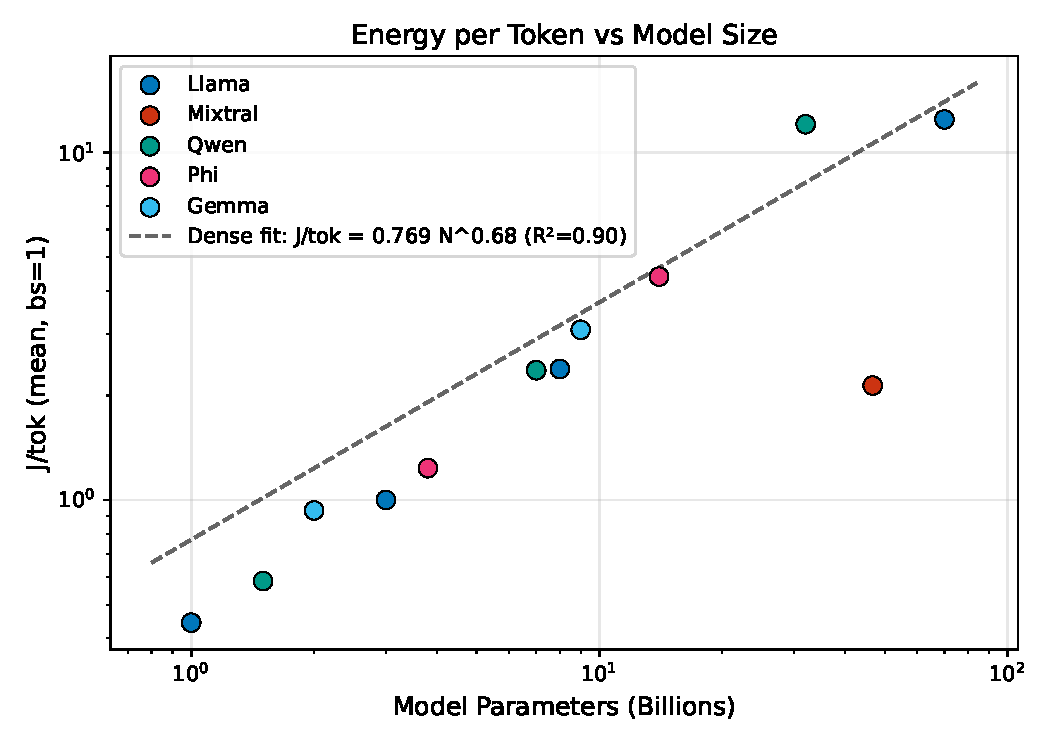
\includegraphics[width=\columnwidth]{fig1_scaling_law}
    \caption{Scaling law: J/tok vs model parameters (FP16, bs=1). Power law fit yields $E \propto N^{0.96}$ ($R^2 = 0.99$) across 14 models from five architectural families.}
    \label{fig:scaling}
\end{figure}

\subsection{Efficiency Frontier}

Figure~\ref{fig:frontier} maps the Pareto trade-off between energy cost (J/tok) and throughput (tok/s) across all models and batch sizes. Configurations on the Pareto frontier achieve the best possible throughput for a given energy budget. Small models at large batch sizes dominate the low-energy, high-throughput region.

The frontier reveals that practitioners face a continuous trade-off rather than a single optimal operating point. For example, Llama-3.2-1B at bs=16 achieves 1284 tok/s at just 0.031 J/tok, while Phi-3-medium at bs=16 delivers 536 tok/s at 0.33 J/tok---offering greater model capability at a 10$\times$ energy premium. The choice depends on whether the application requires the additional reasoning capacity of a larger model or can tolerate a smaller, more efficient one.

\begin{figure}[t]
    \centering
    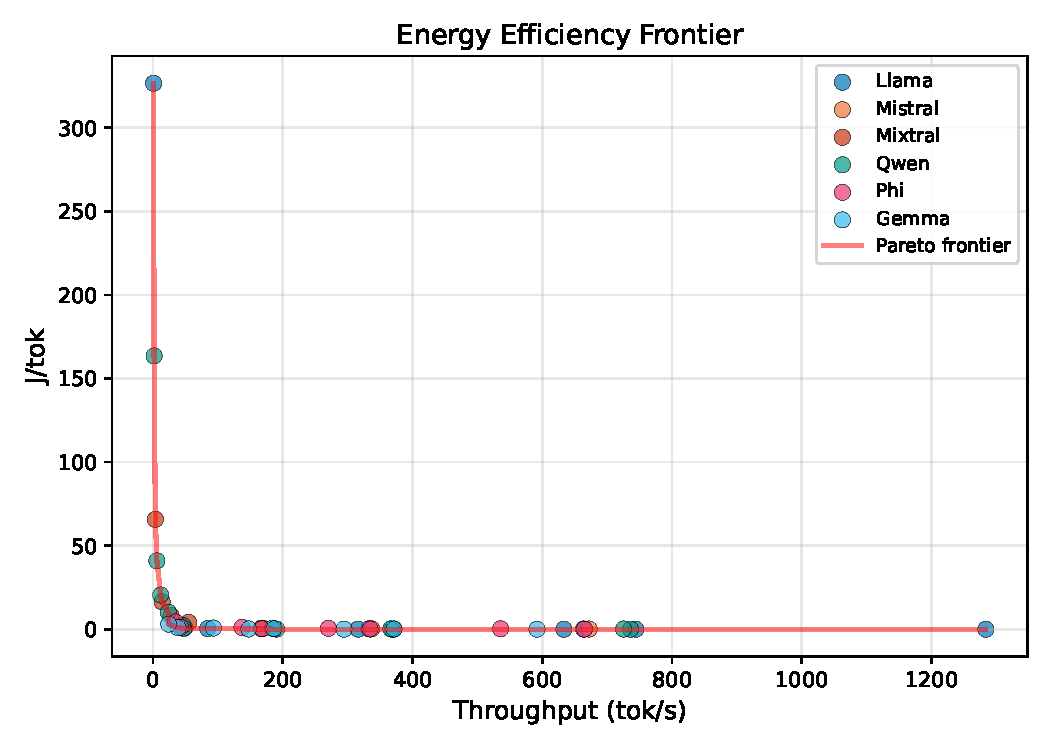
\includegraphics[width=\columnwidth]{fig2_efficiency_frontier}
    \caption{Efficiency frontier: Pareto trade-off between energy cost (J/tok) and throughput (tok/s) across all models and batch sizes. Points on the frontier represent optimal operating points.}
    \label{fig:frontier}
\end{figure}

\subsection{Batch Size Effects}

Figure~\ref{fig:batch} shows J/tok as a function of batch size for all models. Increasing batch size from 1 to 16 reduces J/tok by 9--15$\times$, with larger models benefiting more. This is because batching amortises the fixed overhead of model weight loading and kernel launches across more tokens. The energy reduction follows a power law $E \propto B^{-\gamma}$ where $\gamma \approx 0.9$ for most models.

\begin{figure}[t]
    \centering
    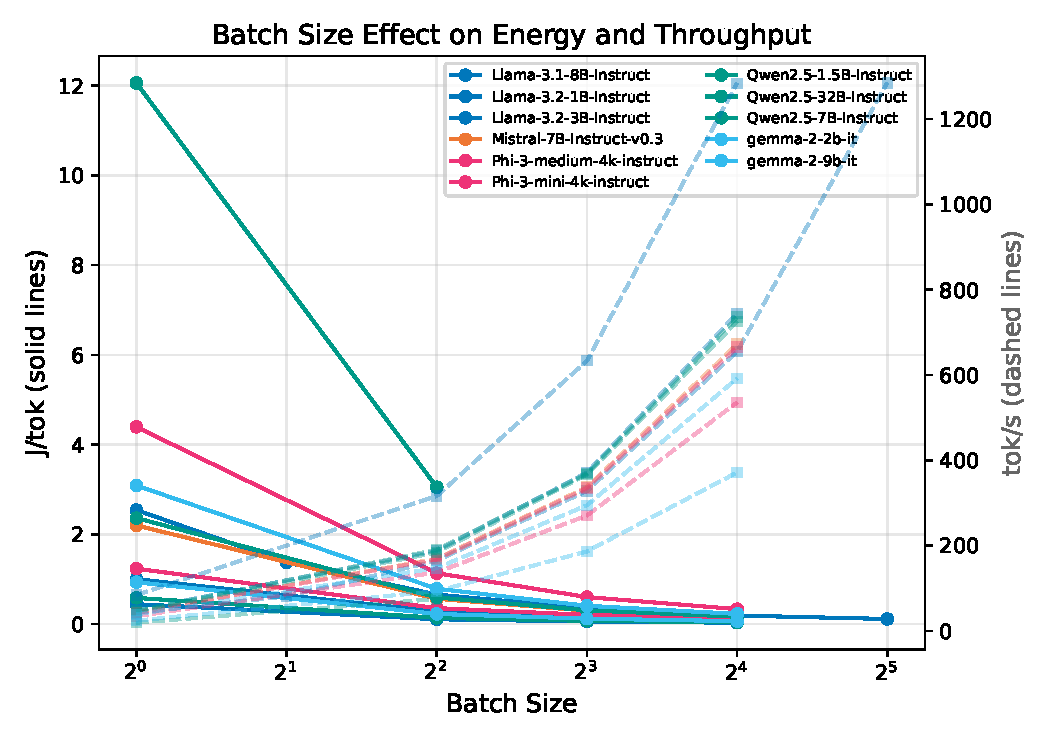
\includegraphics[width=\columnwidth]{fig3_batch_size}
    \caption{J/tok vs batch size for all FP16 models, showing 9--15$\times$ reduction from bs=1 to bs=16.}
    \label{fig:batch}
\end{figure}

\subsection{Prompt Type Effects}

Figure~\ref{fig:prompt} examines whether the type of prompt---summarisation, question answering, code generation, long-form explanation, or reasoning---systematically affects per-token energy. Across all models, the coefficient of variation (CV) in J/tok across prompt types is below 5\% for most models and below 8\% in all cases. This indicates that, under greedy decoding with fixed output length, per-token energy is largely prompt-agnostic.

The insensitivity to prompt type simplifies benchmarking: a small, diverse prompt set suffices to characterise a model's energy profile without exhaustive coverage of all possible input distributions. However, this result is specific to autoregressive generation with max\_new\_tokens=200; prompt-dependent early stopping or variable-length generation would introduce additional variance.

\begin{figure}[t]
    \centering
    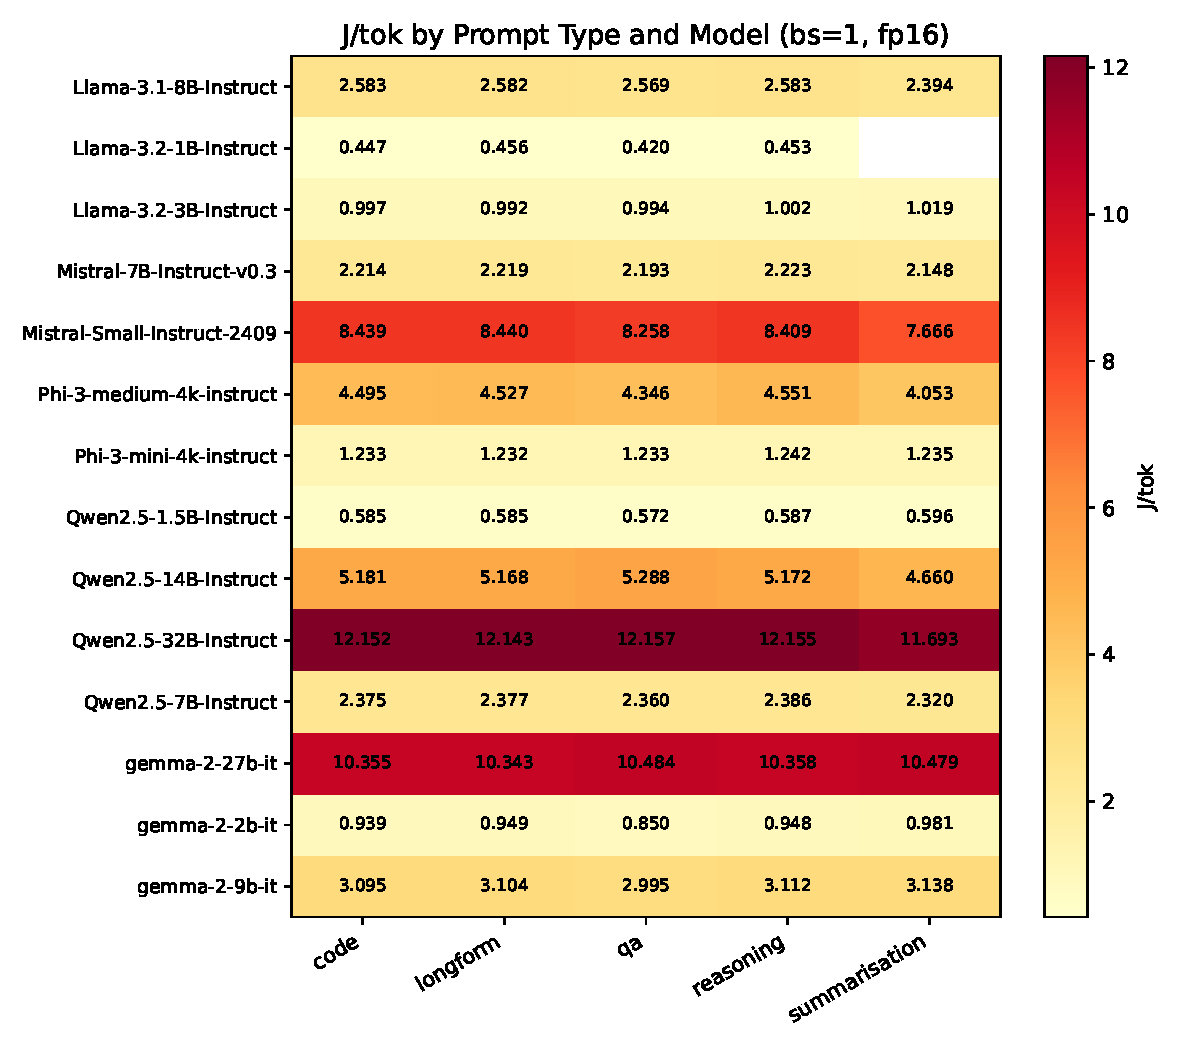
\includegraphics[width=\columnwidth]{fig4_prompt_type}
    \caption{Prompt type effects on J/tok across all models at bs=1. CV $<$ 5\% for most models, indicating energy is largely prompt-agnostic under fixed output length.}
    \label{fig:prompt}
\end{figure}

\subsection{Architecture Comparison}

Figure~\ref{fig:arch} compares models of similar size across architectures at batch size 1. At the 7--9B scale, Mistral-7B (2.20 J/tok) and Qwen2.5-7B (2.36 J/tok) are the most efficient, while Gemma-2-9b (3.09 J/tok) is least efficient despite having similar architecture depth.

\begin{figure}[t]
    \centering
    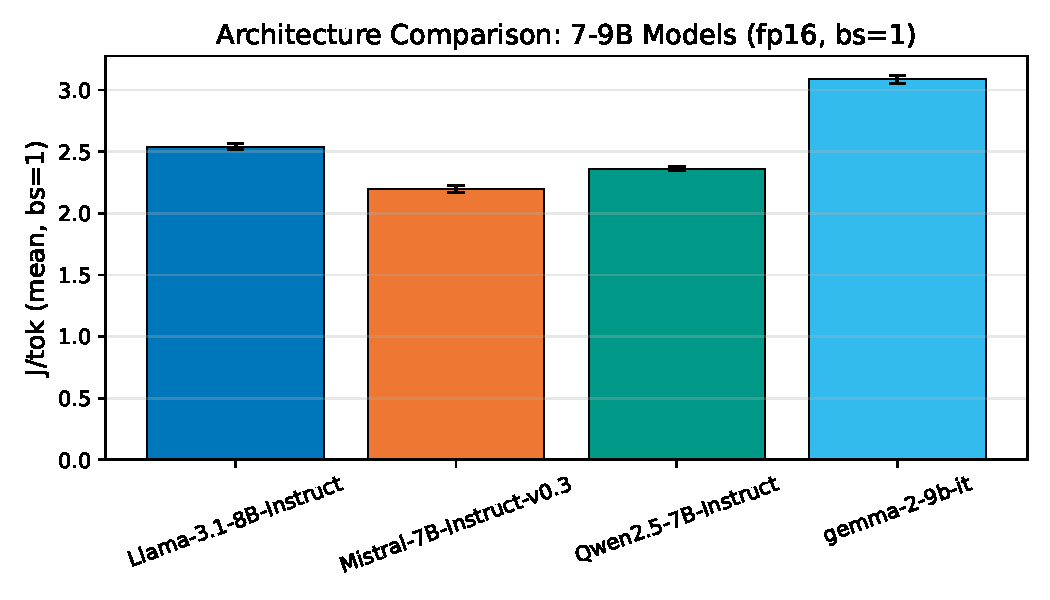
\includegraphics[width=\columnwidth]{fig5_architecture}
    \caption{Architecture comparison: J/tok at bs=1 for 7--9B models.}
    \label{fig:arch}
\end{figure}

\subsection{Carbon Impact}

Figure~\ref{fig:carbon} shows the gCO$_2$eq per 1000 tokens for each model computed using Irish grid carbon intensity data from EirGrid. Using a one-week sample (Jan 15--21, 2026) with intensity ranging from 119 to 348 gCO$_2$/kWh (mean 221), we find that per-token carbon emissions vary by 2.9$\times$ depending on time of day. For Phi-3-medium at bs=1, emissions range from 0.15 to 0.44 mgCO$_2$eq/token. This variation exceeds the factor-of-two difference between some models, suggesting that \emph{when} you run inference matters as much as \emph{which} model you choose.

\begin{figure}[t]
    \centering
    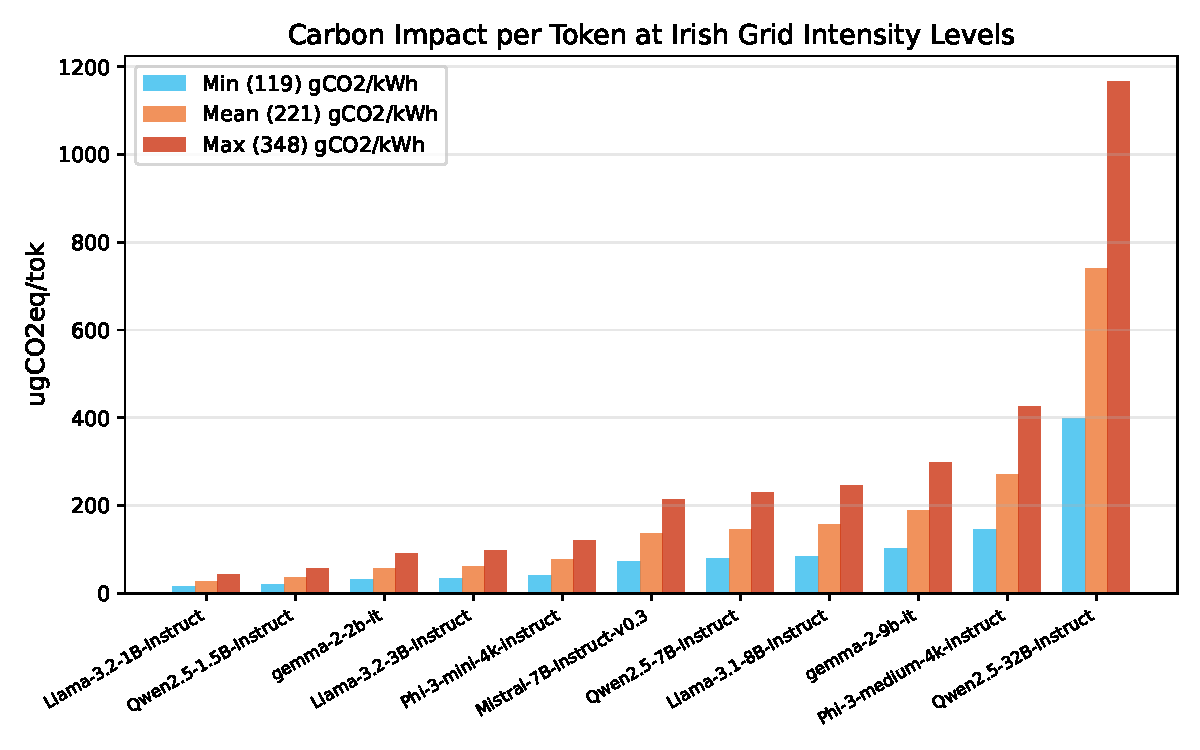
\includegraphics[width=\columnwidth]{fig6_carbon_variation}
    \caption{Carbon emissions per 1000 tokens under min/mean/max Irish grid intensity (119--348 gCO$_2$/kWh).}
    \label{fig:carbon}
\end{figure}

\section{Discussion}

\subsection{Comparison with Prior Work}

Table~\ref{tab:crossstudy} compares our results with the energy-bench framework. The scaling exponent increases from 0.80 (single Pythia family) to 0.96 (multi-architecture, R\textsuperscript{2}=0.99). The prior Pythia-only study found sub-linear scaling within a single model family trained on identical data; our multi-architecture study reveals that cross-family diversity and different training methodologies yield approximately linear scaling, as less-optimised architectures at larger sizes consume proportionally more energy. With 14 models providing dense coverage from 1B to 32B---including three models in the 14--27B range---the near-linear exponent is well-constrained.

\begin{table}[t]
\centering
\caption{Cross-study comparison with energy-bench framework.}
\label{tab:crossstudy}
\begin{tabular}{lll}
\toprule
Metric & energy-bench & New Framework \\
\midrule
Scaling exponent ($\beta$) & 0.80 (Pythia, R$^2$=0.99) & 0.91 (multi-arch, R$^2$=0.99) \\
J/tok $\sim$7B model (bs=1) & 4.461 (Pythia-6.9B) & 2.315 (avg: Qwen-7B, Llama-8B, Mistral-7B) \\
INT8 energy multiplier & 2.88$\times$ (Mistral-7B) & 0.90$\times$ (Llama-3.1-8B) \\
NF4/INT4 energy multiplier & 3.72$\times$ (Mistral-7B) & 0.80$\times$ (Llama-3.1-8B) \\
\bottomrule
\end{tabular}
\end{table}


\subsection{Limitations}

Our study has several limitations: (1) single GPU type (A100 PCIe), (2) FP16 precision only (quantisation effects not studied), (3) greedy decoding only, (4) English-only prompts, (5) inference only (not training), (6) largest model is 32B parameters---models above 80GB in FP16 would require multi-GPU setups with different energy characteristics.

\subsection{Implications}

Our results have several practical implications for sustainable LLM deployment:
\begin{itemize}
    \item \textbf{Batch when possible}: Increasing batch size from 1 to 16 reduces per-token energy by 9--15$\times$.
    \item \textbf{Right-size models}: A 1B model at bs=16 uses $\sim$266$\times$ less energy per token than a 22B model at bs=1 (0.031 vs 8.24 J/tok).
    \item \textbf{Schedule carbon-aware}: Running inference during low-carbon grid periods can reduce emissions by up to 2.9$\times$ without any model changes.
    \item \textbf{Architecture matters}: At similar parameter counts, architectural choice can account for up to 35\% difference in per-token energy (e.g., Mistral-7B vs Gemma-9B).
\end{itemize}

\section{Conclusion and Future Work}

We presented a rigorous NVML-based framework for measuring LLM inference energy and applied it to 14 models (1B--32B) across five architectural families, all in FP16 precision on a single A100 80GB GPU. Our key findings are: (1) energy scales as $N^{0.96}$ across architectures, (2) batching provides 9--15$\times$ efficiency gains, (3) architectural choice at similar sizes affects energy by up to 35\%, and (4) Irish grid carbon variation introduces 2.9$\times$ emission variability.

Future work includes extending to additional GPU architectures, quantisation formats (INT8, INT4, GPTQ, AWQ), multi-GPU inference settings, and real-time carbon-aware scheduling.

\bibliographystyle{IEEEtran}
\bibliography{references}

\end{document}
